% article example for classicthesis.sty
\documentclass[10pt,a4paper]{article} % KOMA-Script article scrartcl
\usepackage{import}
\usepackage{xifthen}
\usepackage{pdfpages}
\usepackage{transparent}
\newcommand{\incfig}[1]{%
    \def\svgwidth{\columnwidth}
    \import{./figures/}{#1.pdf_tex}
}
\usepackage{lipsum}     %lorem ipsum text
\usepackage{titlesec}   %Section settings
\usepackage{titling}    %Title settings
\usepackage[margin=10em]{geometry}  %Adjusting margins
\usepackage{setspace}
\usepackage{listings}
\usepackage{amsmath}    %Display equations options
\usepackage{amssymb}    %More symbols
\usepackage{xcolor}     %Color settings
\usepackage{pagecolor}
\usepackage{mdframed}
\usepackage[spanish]{babel}
\usepackage[utf8]{inputenc}
\usepackage{longtable}
\usepackage{multicol}
\usepackage{graphicx}
\graphicspath{ {./Images/} }
\setlength{\columnsep}{1cm}

% ====| color de la pagina y del fondo |==== %
\pagecolor{black}
\color{white}



\begin{document}
    %========================{TITLE}====================%
    \title{\rmfamily\normalfont\spacedallcaps{ Manejo de excepciones }}
    \author{\spacedlowsmallcaps{Rodrigo Castillo}}
    \date{\today}

    \maketitle


     % ====| Loguito |==== %
    
\includegraphics[width=0.1\linewidth]{negro_cara.png}
    %=======================NOTES GOES HERE===================%

    \section{por que manejo de excepciones?}
        porque a veces cuando manejamos apis podemos tener varios
        errores locos, es bueno poder manejarlos
        \\ el manejo de las excepciones nos permite saber el tipo de output y
        programar respecto a esto.
        \\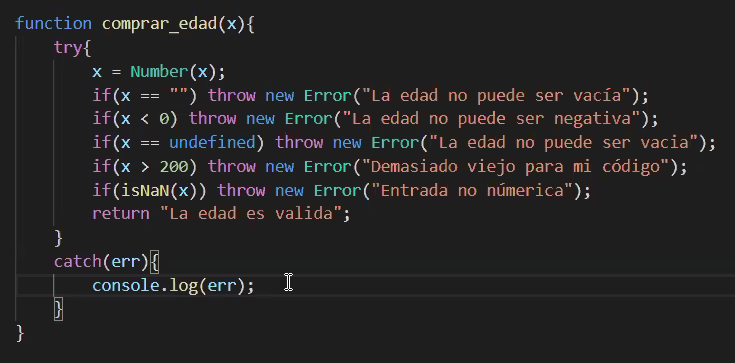
\includegraphics[width=0.8\linewidth]{try_catch.png}
        \\a esto le podemos agregar un final
        \\ 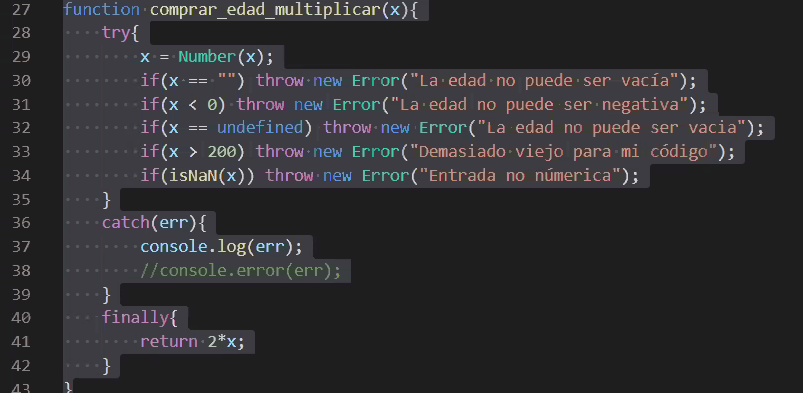
\includegraphics[width=0.8\linewidth]{erroresquedejanavanzar.png}
        \\
    \section{Objetos}
       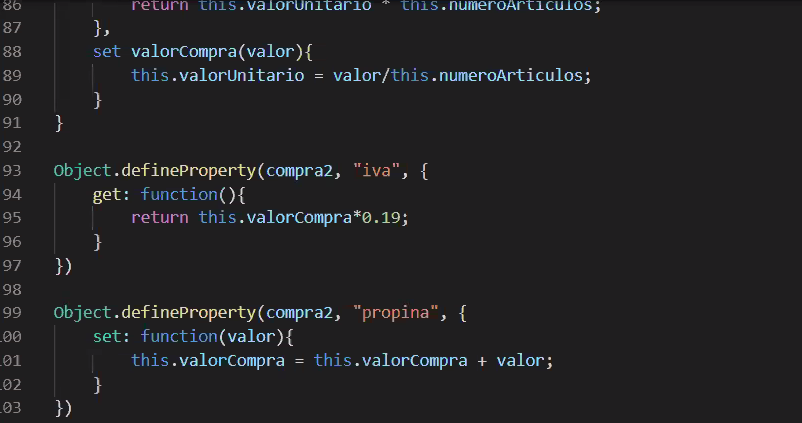
\includegraphics[width=0.8\linewidth]{objetos.png}
       \\
       los objetos tambien pueden tener funciones
       \\
       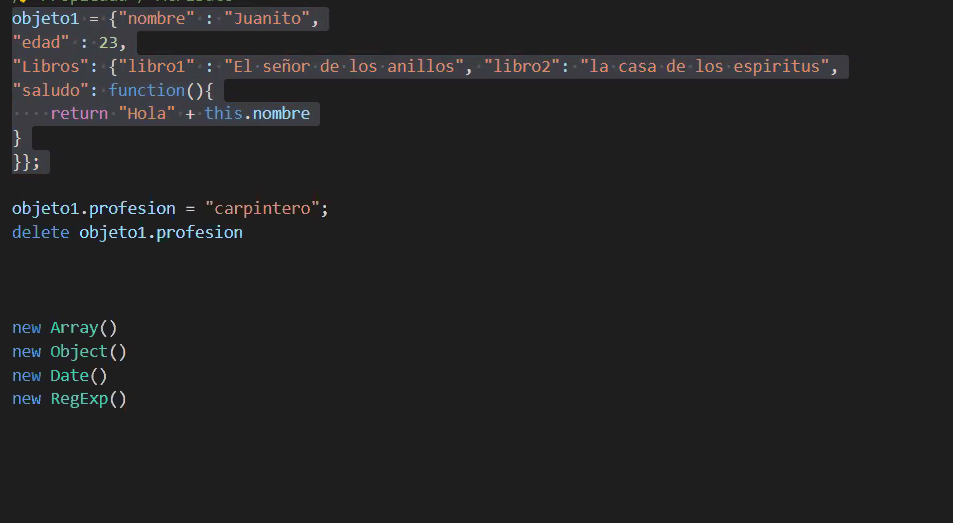
\includegraphics[width=0.8\linewidth]{clase.png}
       \\
    \section{tipos de variables}
        \\
        hay 3 tipos de hacer variables
        \begin{enumerate}
            \item {var}
            \item {let}
            \item {const}
        \end{enumerate}
        \\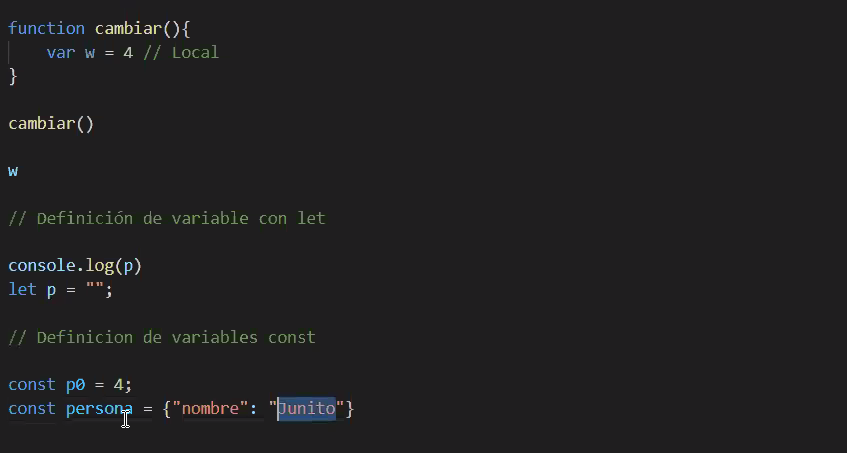
\includegraphics[width=0.8\linewidth]{variables.png}
        \\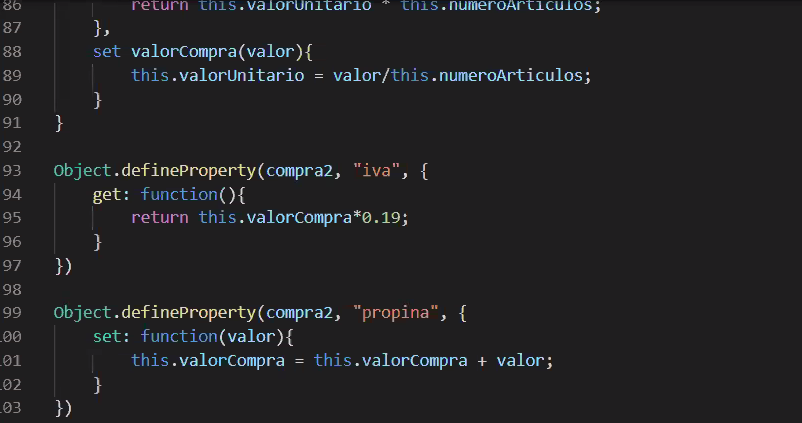
\includegraphics[width=0.8\linewidth]{objetos.png}
        \\
        \section{tarea}
            hacer la tarea del objeto bla bla bla









    %=======================NOTES ENDS HERE===================%

    % bib stuff
    \nocite{*}
    \addtocontents{toc}{\protect\vspace{\beforebibskip}}
    \addcontentsline{toc}{section}{\refname}
    \bibliographystyle{plain}
    \bibliography{../Bibliography}
\end{document}
